\section{Auswertung}
\label{sec:Auswertung}

\subsection{Vorbereitung und technische Daten}

\begin{table}
    \centering
    \caption{Technische Daten.}
    \label{tab:techDaten}
    \begin{tabular}{l l c l}
        \toprule
        Medium          & Größe                 & Variable      & Wert                                      \\
        \midrule
        Flüssigkeit     & Dichte                & $\rho$        & $\SI{1.15}{\gram\per\cubic\centi\meter}$  \\
                        & Schallgeschwindigkeit & $c_\text{L}$  & $\SI{1800}{\meter\per\second}$            \\
                        & Viskosität            & $\eta$        & $\SI{12}{\milli\pascal\second}$           \\
        Prisma          & Schallgeschwindigkeit & $c_\text{P}$  & $\SI{2700}{\meter\per\second}$            \\
                        & Vorlaufstrecke        & $l$           & $\SI{30.7}{\milli\meter}$                 \\
        Strömungsrohr   & Innendurchmesser      & $d_\text{i}$  & $\SI{10}{\milli\meter}$                   \\
                        & Außendurchmesser      & $d_\text{a}$  & $\SI{15}{\milli\meter}$                   \\
        \bottomrule
    \end{tabular}
\end{table}

Das verwendete Prisma hat drei verschiedene (Prisma-)Winkel $\theta$, unter denen die Strömung in den Rohren untersucht wird. 
Der daraus resultierende Doppler-Winkel $\alpha$ wird über 
\begin{equation*}
    \alpha=\SI{90}{\degree}-\arcsin \Bigl(\sin \theta \cdot \frac{c_\text{L}}{c_\text{P}}\Bigr)
\end{equation*}
berechnet. Die Kenndaten $c_\text{L}$ und $c_\text{P}$ sind in Tabelle \ref{tab:techDaten} zu finden.

Die Werte für die Winkel sind in Tabelle \ref{tab:Winkel} aufgeführt.
\begin{table}
    \centering
    \caption{Prisma- und Doppler-Winkel.}
    \label{tab:Winkel}
    \begin{tabular}{c c}
        \toprule
        Prisma-Winkel $\theta$ & Doppler-Winkel $\alpha$ \\
        \midrule
        $\SI{15}{\degree}$ & $\SI{80.064}{\degree}$ \\        
        $\SI{30}{\degree}$ & $\SI{70.529}{\degree}$ \\
        $\SI{45}{\degree}$ & $\SI{61.874}{\degree}$ \\        
        \bottomrule
    \end{tabular}
\end{table}

\subsection{Die Strömungsgeschwindigkeit in Abhängigkeit des Doppler-Winkels}

\begin{table}
    \centering
    \caption{Messwerte.}
    \label{tab:1Mess}
    \begin{tabular}{c c c c c c c}
        \toprule
            & \multicolumn{6}{c}{Prisma-Winkel $\theta$} \\
        \cmidrule(lr){2-7}
            & \multicolumn{2}{c}{$\SI{15}{\degree}$} & \multicolumn{2}{c}{$\SI{30}{\degree}$} & \multicolumn{2}{c}{$\SI{45}{\degree}$} \\
        RPM & $\Delta \nu_\text{max}\,/\,\si{\hertz}$ & $\Delta \nu_\text{mean}\,/\,\si{\hertz}$ & $\Delta \nu_\text{max}\,/\,\si{\hertz}$ & $\Delta \nu_\text{mean}\,/\,\si{\hertz}$ & $\Delta \nu_\text{max}\,/\,\si{\hertz}$ & $\Delta \nu_\text{mean}\,/\,\si{\hertz}$ \\
        \midrule
        2000 &  90 &  49 & 120 &  73 & -105 & -61  \\
        2800 &  94 &  61 & 235 & 134 & -145 & -85  \\
        3600 & 135 &  85 & 375 & 208 & -220 & -122 \\
        4400 & 200 & 110 & 555 & 293 & -330 & -165 \\
        5200 & 290 & 146 & 820 & 415 & -470 & -232 \\
        \bottomrule
    \end{tabular}
\end{table}

Die aufgenommenen Messwerte sind in Tabelle \ref{tab:1Mess} zu finden. 
Der Rechner für die Datenaufnahme zeigt jeweils zwei Werte an für die Frequenzverschiebung: Zum einen die maximale, zum 
anderen die gemittelte Frequenzdifferenz. 
Beide Werte sind für die Auswertung aufgenommen worden. 

Die Zentrifugalpumpe gibt hierbei ihre Umdrehungen pro Zeiteinheit in $\mathrm{rpm}$; es wird erwartet, dass die Umdrehungszahl 
proportional zur Strömungsgeschwindigkeit der Flüssigkeit ist. 
In den Abbildungen \ref{fig:exp15}, \ref{fig:exp30} und \ref{fig:exp45} sind die Frequenzverschiebungen gegen die Umdrehungszahl aufgetragen. 
In den nebenstehenden Abbildungen \ref{fig:theo15}, \ref{fig:theo30} und \ref{fig:theo45} ist die Frequenzverschiebung 
gegen die Strömungsgeschwindigkeit $v$ aufgetragen, die über die Formel 
\begin{equation*}
    \Delta \nu=2 \nu_0 \frac{v}{c} \cos \alpha
\end{equation*}
berechnet wird. Verwendet wird eine $\SI{2}{\mega\hertz}$-Sonde, deshalb ist $\nu_0=\SI{2}{\mega\hertz}$. 

Aufgrund des als proportional angenommenen Zusammenhangs zwischen der Drehzahl der Pumpe und der Strömungsgeschwindigkeit 
wird angenommen, dass die Messpunkte in den Graphiken \ref{fig:15}, \ref{fig:30} und \ref{fig:45} einen ähnlichen Verlauf haben. 

\begin{figure}
    \centering
    \begin{subfigure}{0.48\textwidth}
        \centering
        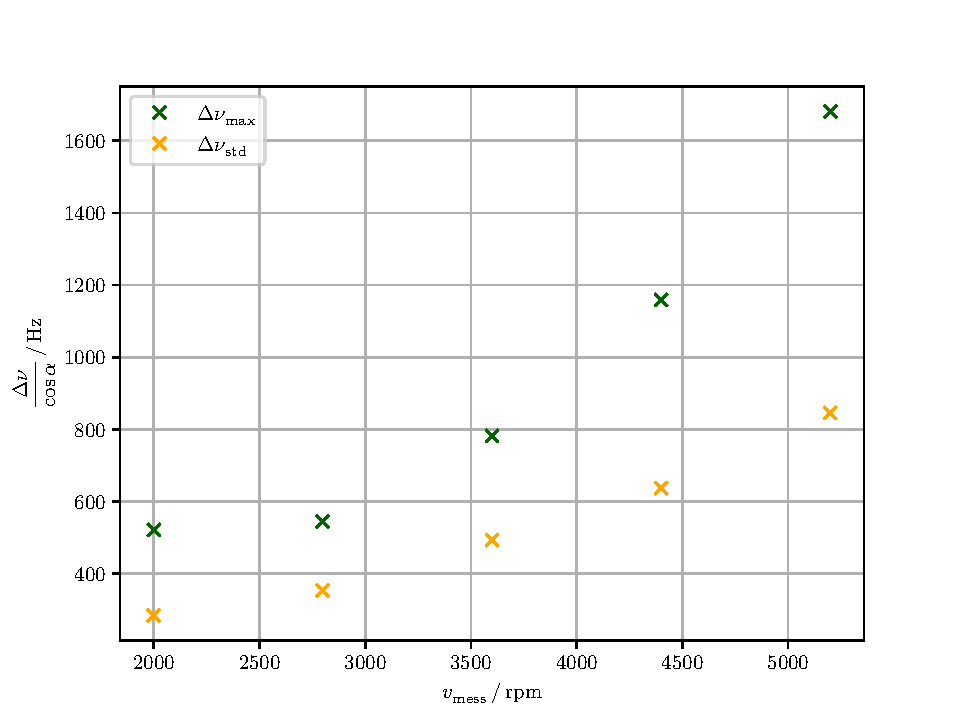
\includegraphics[height=5.0cm]{plots/15_2.pdf}
        \caption{Mit der Geschwindigkeit, die durch die Zentrifugalpumpe gegeben wird.}
        \label{fig:exp15}
    \end{subfigure}
    \begin{subfigure}{0.48\textwidth}
        \centering
        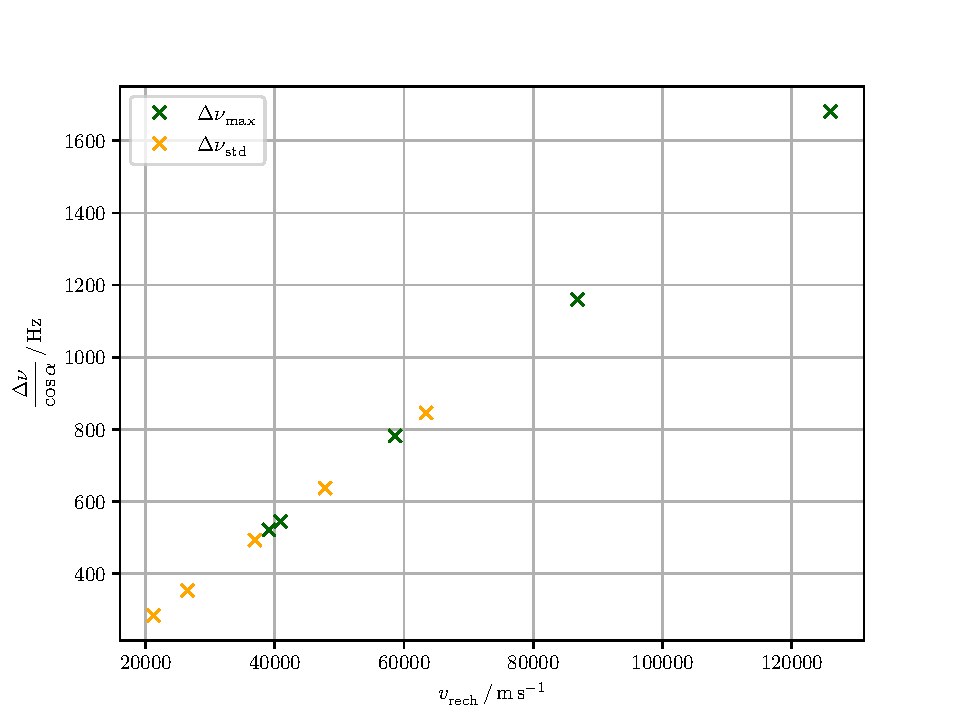
\includegraphics[height=5.0cm]{plots/15_1.pdf}
        \caption{Theoretisch berechnete Strömungsgeschwindigkeit.}
        \label{fig:theo15}
    \end{subfigure}
    \caption{Graphiken zum Prisma-Winkel $\theta=\SI{15}{\degree}$.}
    \label{fig:15}
\end{figure}
\begin{figure}
    \centering
    \begin{subfigure}{0.48\textwidth}
        \centering
        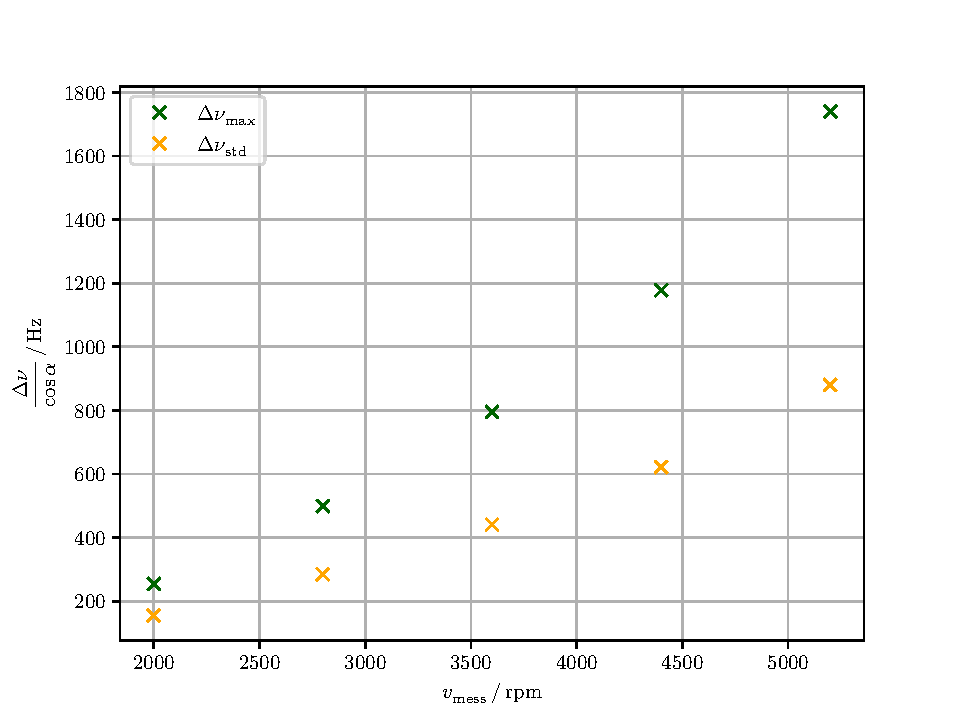
\includegraphics[height=5.0cm]{plots/30_2.pdf}
        \caption{Mit der Geschwindigkeit, die durch die Zentrifugalpumpe gegeben wird.}
        \label{fig:exp30}
    \end{subfigure}
    \begin{subfigure}{0.48\textwidth}
        \centering
        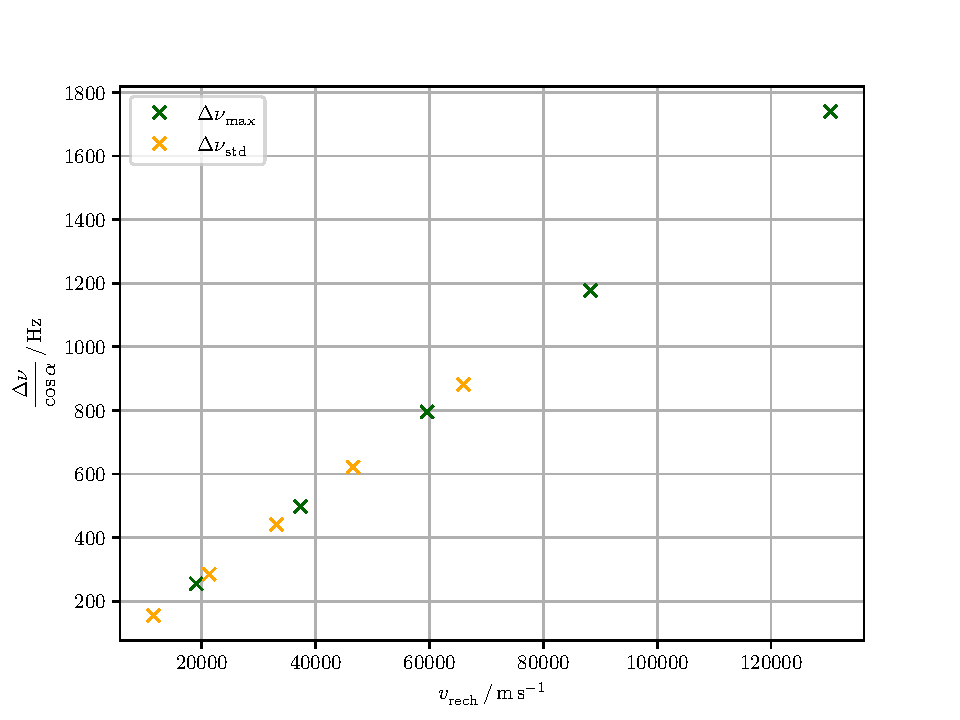
\includegraphics[height=5.0cm]{plots/30_1.pdf}
        \caption{Theoretisch berechnete Strömungsgeschwindigkeit.}
        \label{fig:theo30}
    \end{subfigure}
    \caption{Graphiken zum Prisma-Winkel $\theta=\SI{30}{\degree}$.}
    \label{fig:30}
\end{figure}
\begin{figure}
    \centering
    \begin{subfigure}{0.48\textwidth}
        \centering
        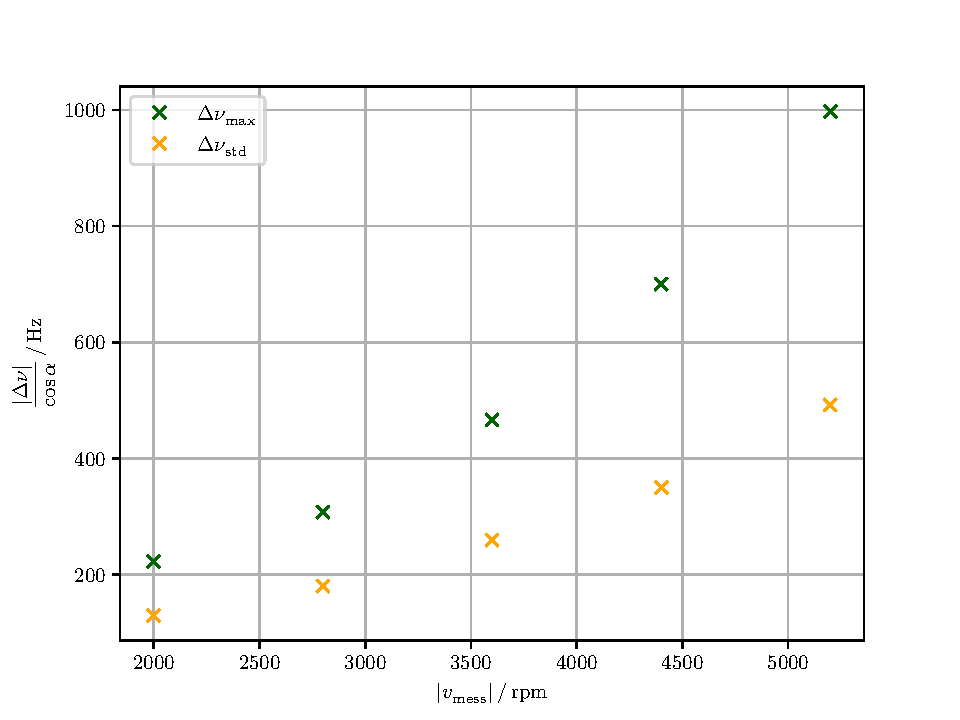
\includegraphics[height=5.0cm]{plots/45_2.pdf}
        \caption{Mit der Geschwindigkeit, die durch die Zentrifugalpumpe gegeben wird.}
        \label{fig:exp45}
    \end{subfigure}
    \begin{subfigure}{0.48\textwidth}
        \centering
        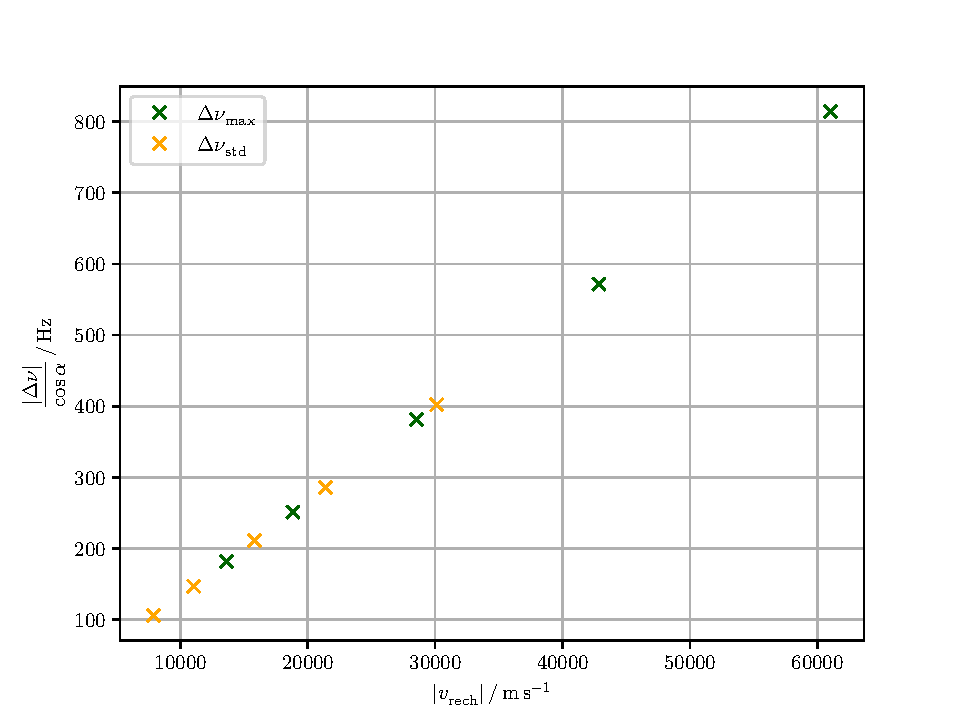
\includegraphics[height=5.0cm]{plots/45_1.pdf}
        \caption{Theoretisch berechnete Strömungsgeschwindigkeit.}
        \label{fig:theo45}
    \end{subfigure}
    \caption{Graphiken zum Prisma-Winkel $\theta=\SI{45}{\degree}$.}
    \label{fig:45}
\end{figure}

\subsection{Strömungsprofil der Doppler-Flüssigkeit}

Hier schreibe ich noch ein paar Worte zu der Messtiefe, warum wir so gemessen haben, wie wir gemessen haben. 
(Also Messtiefe in Sekunden entspricht einer bestimmten Dicke im Festkörper etc -- wenn du das nicht schon in der Theorie machst)
Und dann verweise ich noch auf die Abbildungen nach Schema F. 

\begin{table}
    \centering
    \caption{Messwerte bei einer Pumpleistung von $70\,\%$.}
    \label{tab:70percent}
    \begin{tabular}{c c c}
        \toprule
        Messtiefe in $\si{\micro\second}$ & Strömungsgeschwindigkeit in $\si{\centi\meter\per\second}$ & Streuintensität in $\SI{e3}{\volt\squared\per\second}$ \\
        \midrule
        12.0 & 44.6 &  19 \\
        12.5 & 44.6 &  60 \\
        13.0 & 54.1 & 115 \\
        13.5 & 63.6 & 170 \\
        14.0 & 73.2 & 230 \\
        14.5 & 85.9 & 270 \\
        15.0 & 89.1 & 300 \\
        15.5 & 92.3 & 330 \\
        16.0 & 85.9 & 400 \\
        16.5 & 70.0 & 450 \\
        17.0 & 57.3 & 450 \\
        17.5 & 47.7 & 310 \\
        18.0 & 44.6 & 200 \\
        18.5 & 50.9 & 110 \\
        19.0 & 60.5 &  90 \\
        19.5 & 60.5 & 100 \\
        \bottomrule
    \end{tabular}
\end{table}

\begin{table}
    \centering
    \caption{Messwerte bei einer Pumpleistung von $45\,\%$.}
    \label{tab:45percent}
    \begin{tabular}{c c c}
        \toprule
        Messtiefe in $\si{\micro\second}$ & Strömungsgeschwindigkeit in $\si{\centi\meter\per\second}$ & Streuintensität in $\SI{e3}{\volt\squared\per\second}$ \\
        \midrule
        12.0 & 47.7 &   7 \\
        12.5 & 27.0 &  30 \\
        13.0 & 27.0 &  80 \\
        13.5 & 31.8 & 100 \\
        14.0 & 35.0 & 170 \\
        14.5 & 38.2 & 230 \\
        15.0 & 41.4 & 250 \\
        15.5 & 41.4 & 280 \\
        16.0 & 38.2 & 300 \\
        16.5 & 31.8 & 330 \\
        17.0 & 28.6 & 300 \\
        17.5 & 25.5 & 200 \\
        18.0 & 25.5 & 100 \\
        18.5 & 28.6 &  50 \\
        19.0 & 30.0 &  50 \\
        19.5 & 30.0 &  60 \\
        \bottomrule
    \end{tabular}
\end{table}

\begin{figure}
    \centering
    \begin{subfigure}{0.48\textwidth}
        \centering
        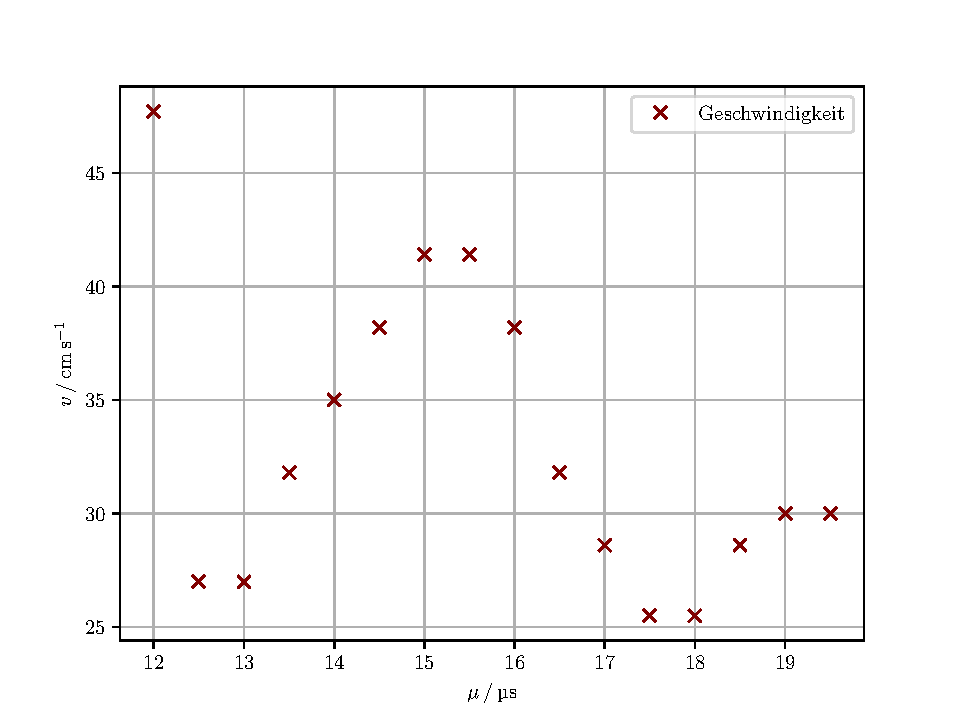
\includegraphics[height=5.0cm]{plots/45velocity.pdf}
        \caption{Mit der Geschwindigkeit, die durch die Zentrifugalpumpe gegeben wird.}
        \label{fig:45velo}
    \end{subfigure}
    \begin{subfigure}{0.48\textwidth}
        \centering
        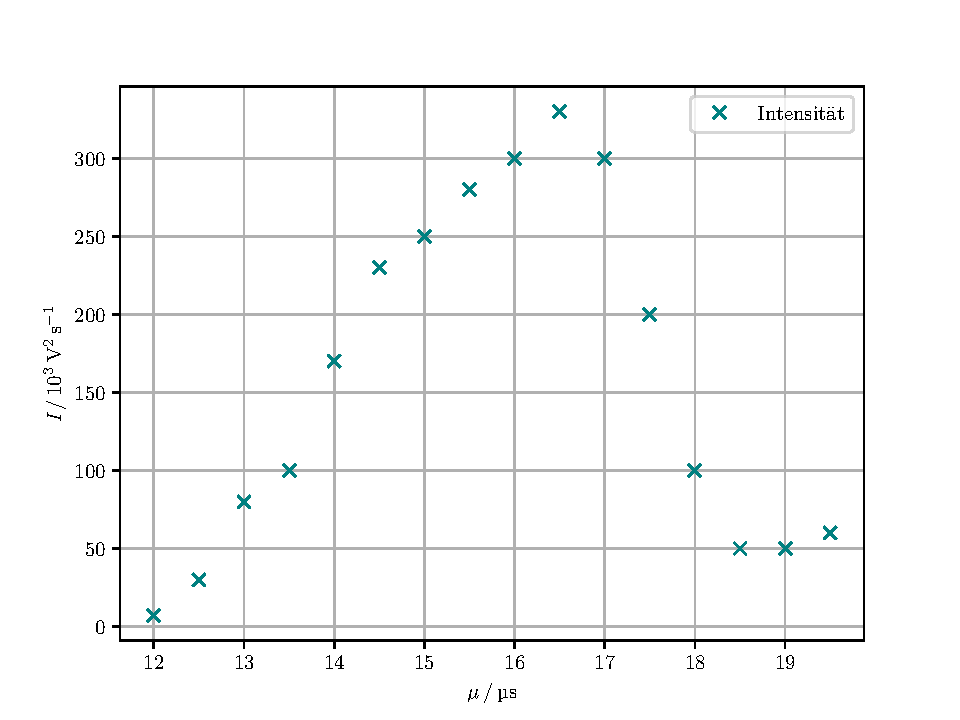
\includegraphics[height=5.0cm]{plots/45intensity.pdf}
        \caption{Theoretisch berechnete Strömungsgeschwindigkeit.}
        \label{fig:45inten}
    \end{subfigure}
    \caption{Die bei $45\,\%$ Pumpleistung aufgenommenen Messpunkte.}
    \label{fig:45vi}
\end{figure}

\begin{figure}
    \centering
    \begin{subfigure}{0.48\textwidth}
        \centering
        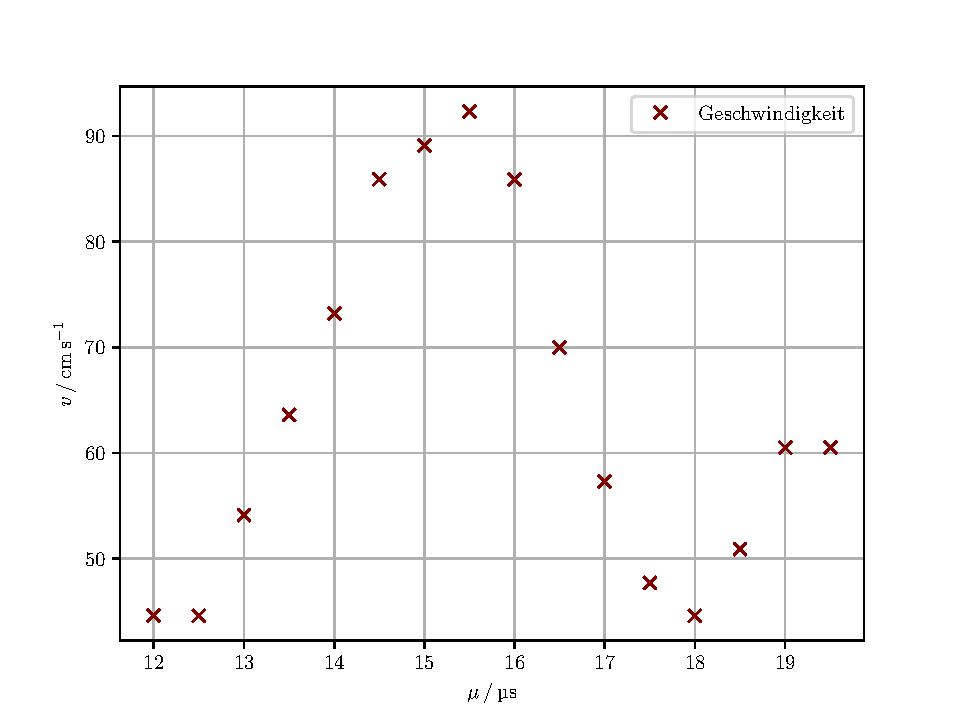
\includegraphics[height=5.0cm]{plots/70velocity.pdf}
        \caption{Mit der Geschwindigkeit, die durch die Zentrifugalpumpe gegeben wird.}
        \label{fig:70velo}
    \end{subfigure}
    \begin{subfigure}{0.48\textwidth}
        \centering
        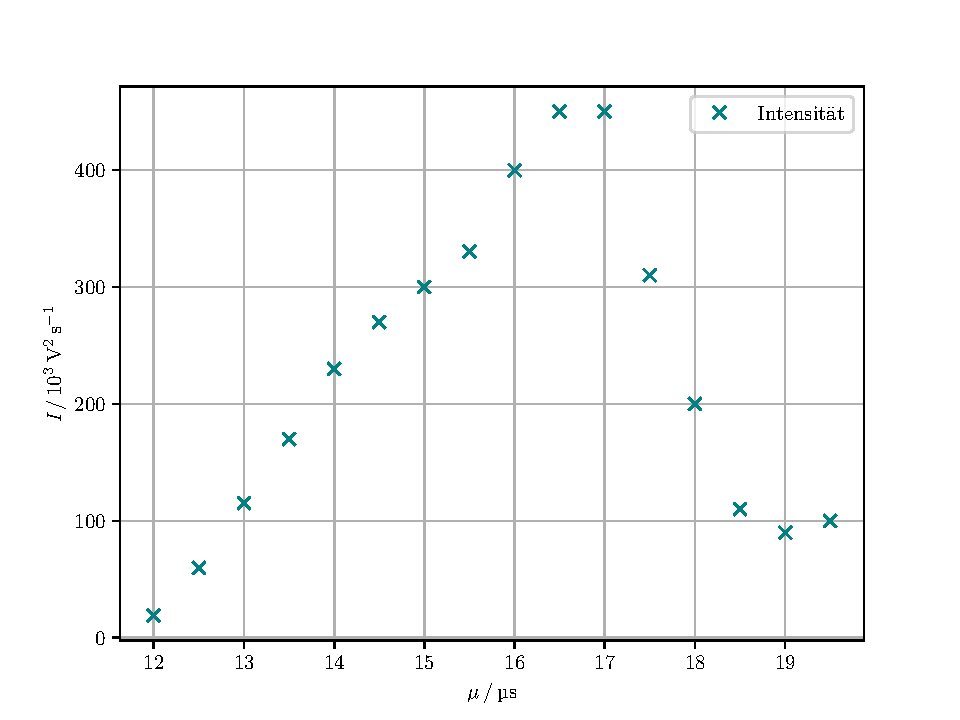
\includegraphics[height=5.0cm]{plots/70intensity.pdf}
        \caption{Theoretisch berechnete Strömungsgeschwindigkeit.}
        \label{fig:70inten}
    \end{subfigure}
    \caption{Die bei $70\,\%$ Pumpleistung aufgenommenen Messpunkte.}
    \label{fig:70vi}
\end{figure}